% !TEX root = paper.tex
\chapter{Evaluation} \label{ch:evaluation}

\noindent
We evaluate our approach with the following two research questions:
%
\begin{itemize}
	%
	\item RQ1. Effectiveness of optimizations: How significantly do the optimizations
	      reduce execution times? (\cref{ch:evaluation:rq1})
	      %
	\item RQ2. Effectiveness as a testing oracle: How many real-world bugs can be
	      detected using the semantics as a testing oracle? (\cref{ch:evaluation:rq2})
	      %
\end{itemize}
%
To facilitate the execution of arbitrary OpenQASM programs using the semantics,
we extracted OCaml code from the Coq mechanization of OpenQASMCore's semantics.
Additionally, we implemented a desugarer in OCaml to transform OpenQASM into
OpenQASMCore.
%
All experiments were conducted on a MacBook Pro, equipped with an M1 Max CPU
and 32GB of memory.
%
We used Qiskit Terra v0.25.3 throughout the evaluation.

\begin{figure}[t]
	\centering
	\begin{subfigure}{0.48\textwidth}
		\centering
		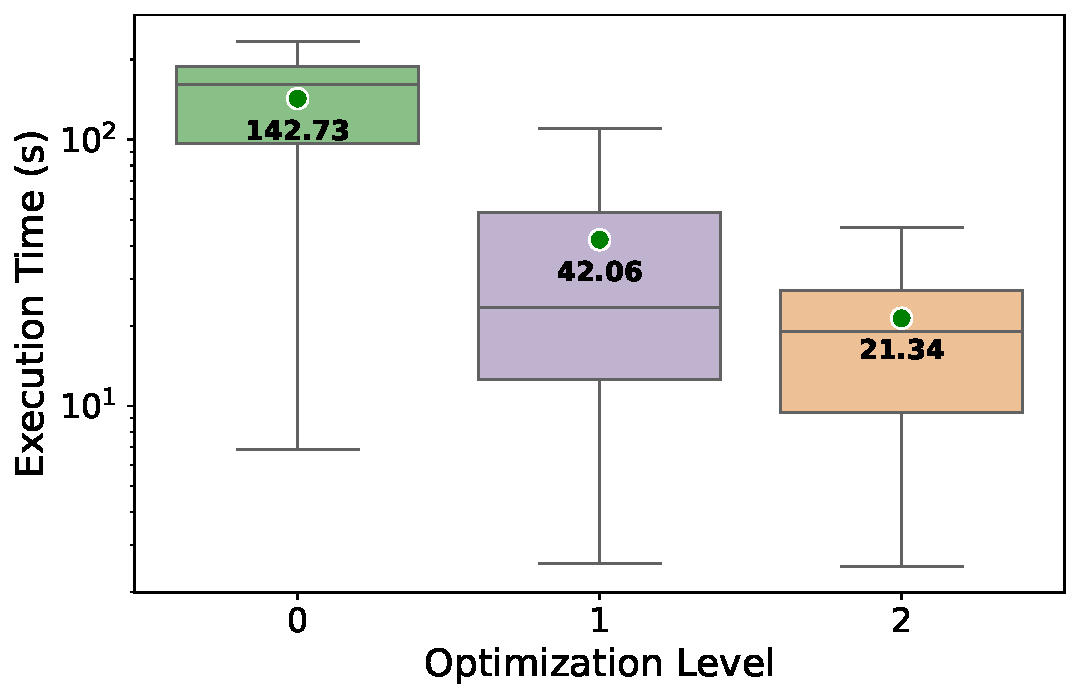
\includegraphics[width=\textwidth]{imgs/opt-bench.pdf}
		\caption{Across different optimization levels}
		\label{fig:result-opt-performance}
	\end{subfigure}
	\hspace{1em}
	\begin{subfigure}{0.48\textwidth}
		\centering
		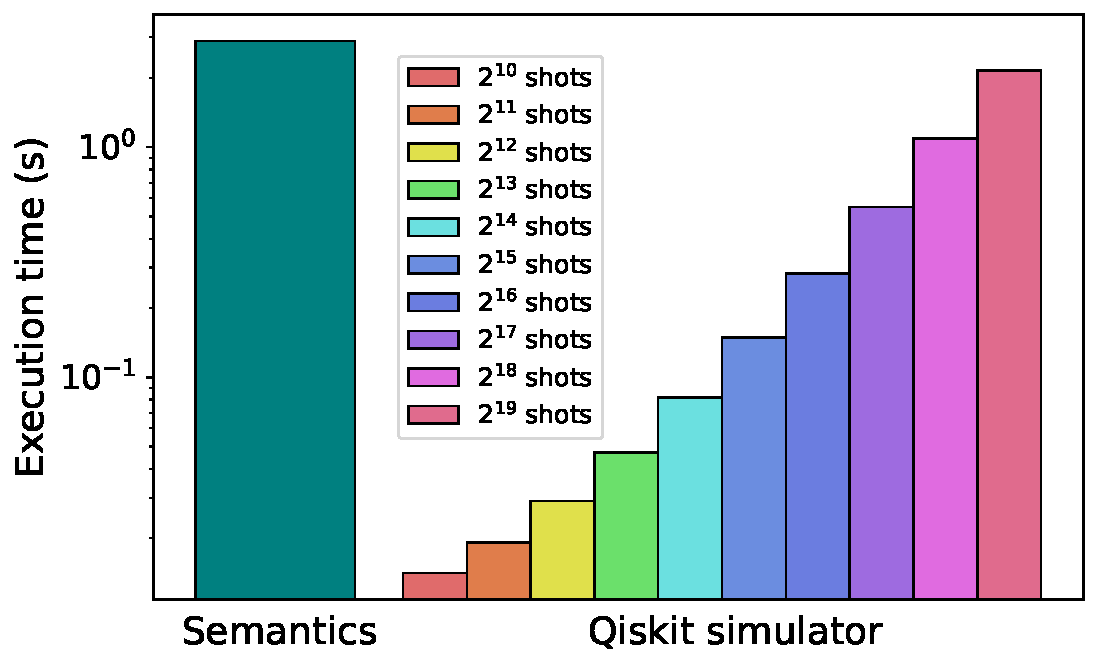
\includegraphics[width=\textwidth]{imgs/sim-bench.pdf}
		\caption{Semantics vs. Qiskit's simulator}
		\label{fig:result-performance}
		\vspace{0.9em}
	\end{subfigure}
	\caption{Execution times of OpenQASM circuits (log scale)}
\end{figure}

\section{RQ1: Effectiveness of Optimizations}
\label{ch:evaluation:rq1}

\noindent
We evaluate the effectiveness of the optimizations in reducing execution times
by comparing three settings: Level 0 (no optimizations), Level 1 (with world
merging), and Level 2 (both optimizations).
%
These optimizations particularly decrease the execution times of dynamic
circuits, which perform mid-circuit measurements, by reducing the creation of
new worlds during measurements.
%
Due to the scarcity of dynamic circuits in available OpenQASM benchmark suites,
we generated 100 random dynamic circuits and used them for evaluation.
%
Each circuit comprises five qubits and average 62.8 random operations, where
each operation is either a reset, a measurement, or a gate chosen from Qiskit's
built-in gate set, consisting of 52 different gates.
%
Additionally, each operation has a 50\% chance of being conditional.
%
By properly setting the probability of selecting each operation, each circuit
has 5.7 measurements and 4.9 resets on average.

Our experimental results indicate a significant reduction in execution times
due to these optimizations.
%
\cref{fig:result-opt-performance} shows a box plot of the execution times across
different settings, with green dots representing average times, annotated in
black text.
%
Two optimizations collectively achieve an average reduction of 85\%.
%
Specifically, world merging achieves an average reduction of 71\%, while
efficient reset leads to a 49\% reduction.
%
World merging is more effective because it can be applied to any statements,
which may create two worlds with the same classical state.
%
This technique would be especially effective in circuits with measurements
considerably more than classical bits, as it limits the number of worlds
regardless of the number of measurements.
%
In contrast, unlike the typical reset, efficient reset does not exponentially
increase the number of worlds with each reset.
%
This benefit exponentially grows with the number of reset statements, making
efficient reset particularly effective for circuits with frequent resets.

To better understand the performance characteristics of the semantics, we
further compare its execution times with those of a real-world simulator.
%
We utilized \C{aer\_simulator} from Qiskit, with parallel execution disabled.
%
For this experiment, we employed 141 circuits from three benchmark suites, in
addition to the 100 randomly generated dynamic circuits.
%
The first suite is OpenQASM 2.0 specification~\cite{openqasm2}, where we
selected six example circuits by excluding one with ten qubits.
%
The second suite is QASMBench~\cite{li2023qasmbench}, where we selected 35
circuits from 81 by excluding those with nine or more qubits and one with eight
qubits.
%
The third suite, Supermarq~\cite{tomesh2022supermarq}, offers eight benchmark
generators, from which we generated 100 circuits.
%
Details on the simulator names and circuit sizes are available in the companion
report~\cite{supp}.

To compare performance, we executed the semantics only once for each circuit,
while we executed the simulator multiple times for each circuit.
%
This approach stems from the fact that our semantics computes the exact
probability distribution, eliminating the need for repeated runs.
%
In contrast, the simulator yields a nondeterministic outcome in each execution,
requiring multiple runs to approximate the probability distribution.

\cref{fig:result-performance} presents the geometric mean of execution times for
the circuits using each method: our semantics with optimization Level 2 or
\C{aer\_simulator}.
%
We employ the geometric mean due to significant variances in execution times
across circuits, with the slowest being 100,000 times longer than the fastest.
%
The left bar in the figure indicates the execution time for the semantics,
while the right bars represent the simulator's execution times, varying by the
number of runs.
%
The results demonstrate that a single semantics run is roughly equivalent in
time to $2^{19}$ simulator runs.
%
However, this does not imply that the semantics' performance is exceedingly
poor, as its capabilities fundamentally differ from those of the simulators,
which cannot compute the exact probability distribution regardless of the
number of runs.

\section{RQ2: Effectiveness as a Tesing Oracle}
\label{ch:evaluation:rq2}

\noindent
To evaluate the effectiveness of our semantics as a testing oracle, we tested a
simulator, \C{aer\_simulator}, provided by Qiskit using the semantics.
%
Simulating an OpenQASM circuit in Qiskit involves three steps:
%
(1) transpilation, which converts OpenQASM code into a circuit in Qiskit's
internal representation,
%
(2) optional optimization passes that transform the circuit, and
%
(3) simulation, which executes the circuit using a simulator.
%
By saying ``we tested a simulator,'' we mean testing all three steps, with the
simulator employed in the third step.
%
We tested steps 2 and 3 separately for effectiveness, utilizing step 1 in both
cases, as steps 2 and 3 rely on step 1.

To test optimization passes with an OpenQASM circuit, we first transpile (step
1) and optimize (step 2) the circuit, with all optimization passes enabled.
%
We then convert the optimized circuit back to OpenQASM code and execute both
the original and the optimized OpenQASM circuits using the semantics.
%
Finally, we compare the resulting probability distributions from both
executions, and any discrepancy indicates a bug in the optimization passes.

To generate circuits that trigger as many optimizations as possible, we
examined the optimization passes and developed a circuit generator tailored to
this task.
%
Below are all the optimization passes in Qiskit, except for
\C{CrosstalkAdaptiveSchedule}, along with the operations we insert into
circuits to activate them.
%
The \C{CrosstalkAdaptiveSchedule} pass is excluded because it optimizes
circuits based on a user-provided hardware description.
%
\begin{itemize}[leftmargin=*]
	%
	\item \C{collect\_cliffords}/\C{collect\_linear\_functions}:
	      %
	      Each of them replaces a block of Clifford/linear gates with a single gate.
	      %
	      We insert a block of Clifford/linear gates.
	      %
	\item \C{commutative\_cancellation}:
	      %
	      It removes a pair of adjacent gates that are self-inverse.
	      %
	      We insert a sequence of self-inverse gates.
	      %
	\item \C{commutative\_inverse\_cancellation}:
	      %
	      It removes a pair of possibly non-adjacent inverse gates by exploiting
	      commutation relations.
	      %
	      We insert a sequence consisting of an arbitrary gate at the beginning, its
	      inverse at the end, and gates commuting with them in between.
	      %
	\item \C{consolidate\_blocks}:
	      %
	      It replaces a sequence of consecutive gates with a single gate.
	      %
	      We insert a sequence of gates.
	      %
	\item \C{cx\_cancellation}:
	      %
	      It removes a pair of adjacent CNOT gates.
	      %
	      We insert a sequence of CNOT gates.
	      %
	\item \C{echo\_rzx\_weyl\_decomposition}:
	      %
	      It rewrites a two-qubit gate using the Weyl decomposition.
	      %
	      We insert a block of two-qubit gates.
	      %
	\item \C{hoare\_opt}:
	      %
	      It applies Hoare logic to selective gates.
	      %
	      We insert a block of gates handled by Hoare logic.
	      %
	\item \C{inverse\_cancellation}:
	      %
	      It removes a pair of adjacent inverse gates.
	      %
	      We insert an arbitrary gate and its inverse. \item
	      \C{optimize\_1q\_commutation}:
	      %
	      It optimizes the circuit by exploiting a 1-qubit gate commuting with a 2-qubit
	      gate.
	      %
	      We insert a 2-qubit gate and a 1-qubit gate commuting with it.
	      %
	\item \C{optimize\_cliffords}:
	      %
	      It replaces a sequence of consecutive Clifford gates over the same qubit with a
	      single gate.
	      %
	      We insert a sequence of Clifford gates over a single qubit.
	      %
	\item \C{optimize\_swap\_before\_measure}:
	      %
	      It removes a SWAP gate followed by a measurement.
	      %
	      We insert a SWAP gate followed by a measurement.
	      %
	\item \C{remove\_diagonal\_gates\_before\_measure}:
	      %
	      It removes a diagonal gate followed by a measurement.
	      %
	      We insert a diagonal gate followed by a measurement.
	      %
	\item \C{remove\_reset\_in\_zero\_state}:
	      %
	      It removes a reset on a qubit in $\ket{0}$ state.
	      %
	      We insert a reset on a qubit in $\ket{0}$ state.
	      %
	\item \C{reset\_after\_measure\_simplification}:
	      %
	      It removes a reset preceded by a measurement.
	      %
	      We insert a reset preceded by a measurement.
	      %
\end{itemize}

To test simulation with an OpenQASM circuit, we transpile (step 1) and then
simulate (step 3) the circuit, with all optimization passes disabled.
%
As the simulator is sampling-based and produces nondeterministic results, we
must compare the outcomes from multiple simulator runs to the probability
distribution computed by the semantics.
%
For this comparison, we employ the chi-square goodness-of-fit
test~\cite{pearson1900criterion}.
%
This test evaluates whether observed outcomes are likely sampled from a given
probability distribution.
%
The p-value computed by the test indicates the likelihood of the observed
outcomes occurring if the null hypothesis (the observations are sampled from
the distribution) is true.
%
A low p-value suggests that the outcomes are improbable under the null
hypothesis, strongly indicating that the observations do not conform to the
expected probability distribution.
%
Consistent with standard statistical hypothesis testing practices, we interpret
a p-value below 0.01 (=1\%) as evidence of divergence between the semantics and
the simulator.

\begin{table}[t]
	\centering
	\caption{Real-world bugs found by our approach}
	\label{table:bugs}
	{\footnotesize
		\begin{tabular}{@{}lllllll@{}}
			\toprule
			ID    & Location      & Platform & Status    & Novelty   & Description                                   \\ \midrule
			Bug 1 & transpilation & Qiskit   & fixed     & new       & losing classical conditionals                 \\
			Bug 2 & optimization  & Qiskit   & fixed     & duplicate & wrong commutation analysis                    \\
			Bug 3 & optimization  & Qiskit   & confirmed & new       & incorrectly optimizing SWAP and measurement   \\
			Bug 4 & optimization  & Qiskit   & confirmed & new       & Hoare optimizer ignoring classical conditions \\
			Bug 5 & optimization  & Qiskit   & confirmed & new       & Hoare optimizer misusing gate cancellation    \\
			Bug 6 & optimization  & staq     & fixed     & new       & losing conditionals                           \\ \bottomrule
		\end{tabular}
	}
\end{table}

Our results demonstrate the effectiveness of the semantics as a testing oracle.
%
We generated 40,000 static circuits and 10,000 dynamic circuits using the
optimization-triggering circuit generator to test both optimization and
simulation.
%
When testing simulation, we ran the simulator 1,024 times for each circuit.
%
From testing, we discovered five bugs in Qiskit, detailed as Bugs 1 to 5 in
\cref{table:bugs}.
%
To the best of our knowledge, this is the first systematic testing to identify
bugs pertained to physical inconsistencies within real-world quantum
programming platforms.

These bugs were identified through optimization testing, with Bug 1 also
detected during simulation testing as it is due to incorrect transpilation.
%
Initially, out of 50,000 circuits, 10,000 (all the dynamic circuits) failed in
optimization testing, and 9,037 yielded p-values below 0.01 in simulation
testing.
%
A manual examination of a few circuits revealed Bug 1.
%
As Bug 1 led to numerous failures, hindering the discovery of other bugs, we
repeated the optimization and simulation testing after fixing Bug 1.
%
This resulted in 2,716 failures in optimization testing and a few circuits with
p-values below 0.01 in simulation testing.
%
Further manual investigation of the failed circuits in optimization testing
identified Bugs 2 to 5:
%
30 failures caused by Bug 2, 99 by Bug 3, 2,586 probably caused by Bug 4, and 1
by Bug 5.
%
While we cannot manually analyze all 2,586 failures, they have conditionals and
persist even when only the \C{hoare\_opt} pass is enabled, leading us to
suspect that all are attributable to Bug 4.
%
Conversely, no additional bugs were identified from circuits with low p-values,
which is consistent with the expectation that approximately 0.01\% of the
circuits should exhibit p-values below 0.01, by definition of a p-value.

Of the identified bugs, four, excluding Bug 2, were previously unknown.
%
Bug 2, although not fixed in the latest release of Qiskit used for our
experiments, had been identified and fixed in the development version.
%
We reported the four new bugs, which were all confirmed by the Qiskit
developers, and Bug 1 was fixed subsequent to our report.

We also conducted experiments with staq, an open-source library for quantum
circuits~\cite{staq}.
%
Since staq provides optimizers but not simulators, we limited our tests to
optimization using the same 50,000 generated circuits.
%
In staq v3.3, we found one previously unknown bug, referred to as Bug 6 in
\cref{table:bugs}, which was subsequently confirmed and fixed by the staq
developers.
%
The circuits used for the experiment are specifically designed for testing the
optimization passes in Qiskit.
%
Therefore, designing a circuit generator tailored for staq's optimization
passes would reveal additional bugs.

\begin{figure}[t]
	\centering
	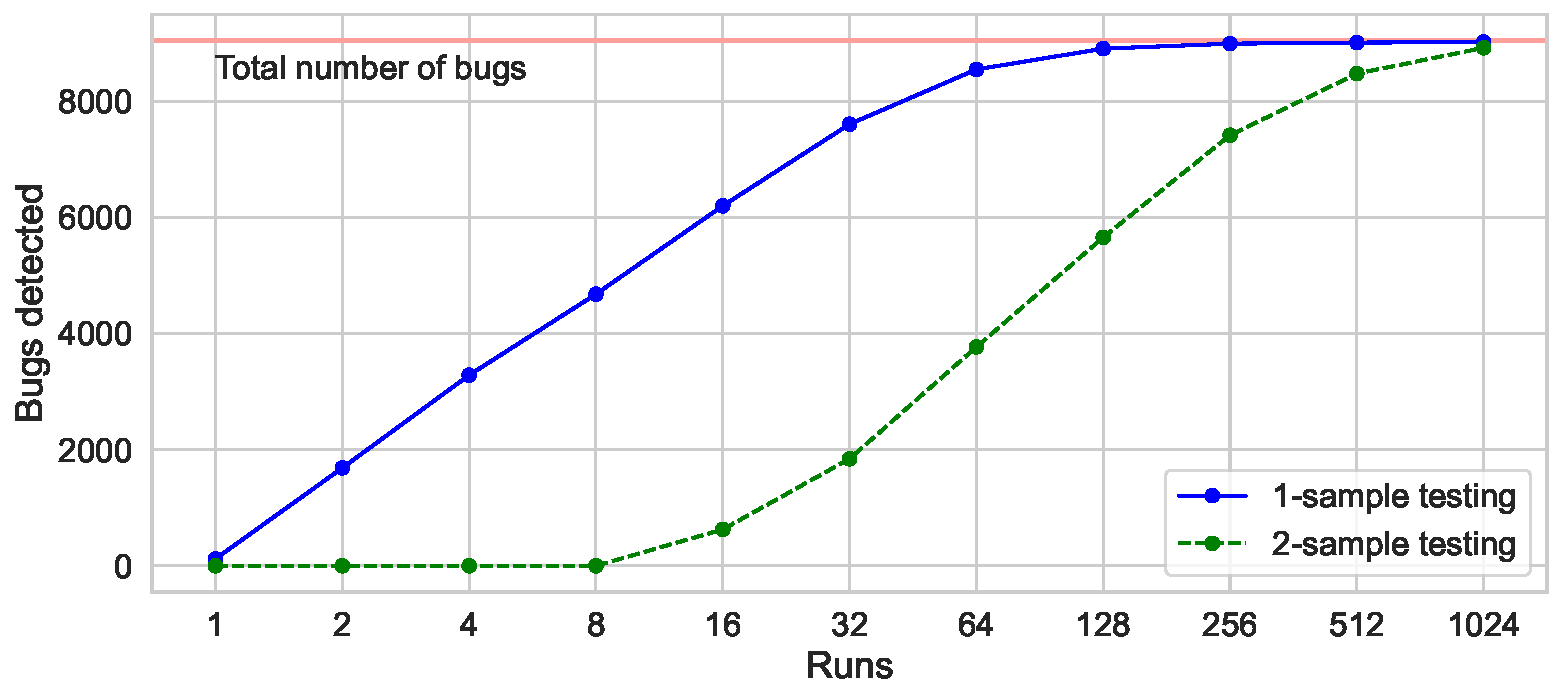
\includegraphics[width=0.64\textwidth]{imgs/1-2-sample-test.pdf}
	\caption{Number of detected bugs per number of simulator runs (x-axis is log scale)}
	\label{fig:onesample}
\end{figure}

We now compare testing simulation using the semantics to existing approaches to
test quantum circuit simulators, \textsc{QDiff}~\cite{wang2022qdiff} and
MorphQ~\cite{paltenghi2023morphq}.
%
\textsc{QDiff} employs a differential testing technique, executing the same
quantum circuit on multiple simulators and checking for output discrepancies.
%
MorphQ, in contrast, utilizes a metamorphic testing technique that generates
multiple semantically equivalent quantum circuits, executing them on a
simulator to compare their outputs.

At first glance, our method may appear similar to the existing ones, as both
methods compare independently-obtained results that should be identical if no
bugs exist.
%
However, our approach directly compares simulator outcomes with the probability
distribution computed by the semantics, known as the \emph{one-sample test} in
statistics.
%
In contrast, \textsc{QDiff} and MorphQ compare two sets of simulator outcomes
to determine if they are sampled from the same probability distribution,
referred to as the \emph{two-sample test}.
%
This distinction arises from the absence of a testing oracle computing the
probability distribution in their approaches.

Our case study demonstrates that our method can detect bugs with significantly
fewer simulator runs than existing approaches, due to the difference in
statistical confidence between one-sample and two-sample tests.
%
We utilized the 9,037 circuits affected by Bug 1 for this study.
%
For varying values of $N$, ranging from 1 to 1,024, we executed each circuit on
the simulator $N$ times.
%
The outcomes were compared with the probability distribution computed by the
semantics using the one-sample test.
%
Additionally, we ran the circuit on the corrected version of the simulator $N$
times, comparing the two sets of outcomes using the two-sample test.
%
In both tests, a p-value below 0.01 indicates successful bug detection.
%
\cref{fig:onesample} presents the results, illustrating that the one-sample test
is more effective than the two-sample test.
%
The x-axis represents $N$, while the y-axis shows the number of circuits in
which Bug 1 is detected.
%
As a larger sample size increases statistical confidence and lowers the
p-value, larger $N$ leads to the discovery of bugs across more circuits.
%
However, regardless of $N$, the one-sample test finds bugs in more circuits
than the two-sample test.

When testing optimization, our approach is even more advantageous than existing
methods.
%
Our method can directly compare distributions without any sampling, while
existing approaches must still rely on the less efficient two-sample test.
